\section{Protocol and Reproduction Details}
\label{sec:audit}

\subsection{Study record}
Before the primary MIPDB evaluation, a study lock recorded the encoder,
preprocessing, statistical specification, HBN manifests, external cohort,
training environment, and all 40 selected checkpoints. Evaluation recorded its
start before extracting features for primary participants. Existing valid
predictions could not be overwritten, and resumed runs had to use the same
inputs. Analysis required exactly one prediction for each head, seed, and
participant: 3,000 predictions in total.

The compact evidence records the primary analysis hash
\texttt{\SourceAnalysisHash} and prediction-inventory hash
\texttt{\PredictionInventoryHash}. These identify the retained result and its
source inventory. They do not replace access to the inventory or provide an
independent public timestamp for the protocol.

The source analyses, figures, and tables are linked by file manifests. Numeric
commands in the manuscript are generated from aggregate results. The editorial
presentation assets use the same retained values with shorter labels; their
manifest records their source files separately. Rebuilding those assets does
not rerun participant-level inference.

\subsection{Interpretation of the decision rule}
The five primary conditions serve different purposes. The minimum cohort size
sets a floor on the evaluation sample. Holm correction addresses the three
seed-level tests, while the bootstrap lower bound requires a positive estimate
when seeds and participants are resampled. The win count and worst-seed floor
limit dependence on favorable training runs. No candidate passed the bootstrap
condition. The multi-query head lost on two seeds, but still met the eight-win
and worst-seed thresholds. Passing those thresholds did not compensate for an
interval containing zero.

\subsection{Earlier and later analyses}
Previously inspected HBN R5 screens motivated candidate families but are
retrospective evidence. NeuralBench-compatible end-to-end runs update the
encoder and provide implementation context, not frozen-probe scores. Neither
is part of the primary MIPDB effect estimate.

The training-size and layer-wise follow-ups reuse the MIPDB cohort after its
first evaluation. Their separate protocol records preserve what was run but
cannot make those participants an untouched holdout again. The ds006780
transfer adds a separate cohort and uses the configuration recorded in
\texttt{configs/research/ds006780\_external\_transfer.json}. Its configuration
hash matches the v5 aggregate execution record, including dataset version
1.0.0 and the pinned source revision. It remains secondary because the
comparison was motivated by earlier findings.

\subsection{Additional primary and layer-wise figures}
Figure~\ref{fig:calibration} summarizes calibration. Figures~\ref{fig:layerwise-depth}
and \ref{fig:layerwise-seed-deltas} show the exploratory depth comparison.

\begin{figure}[!htbp]
  \centering
  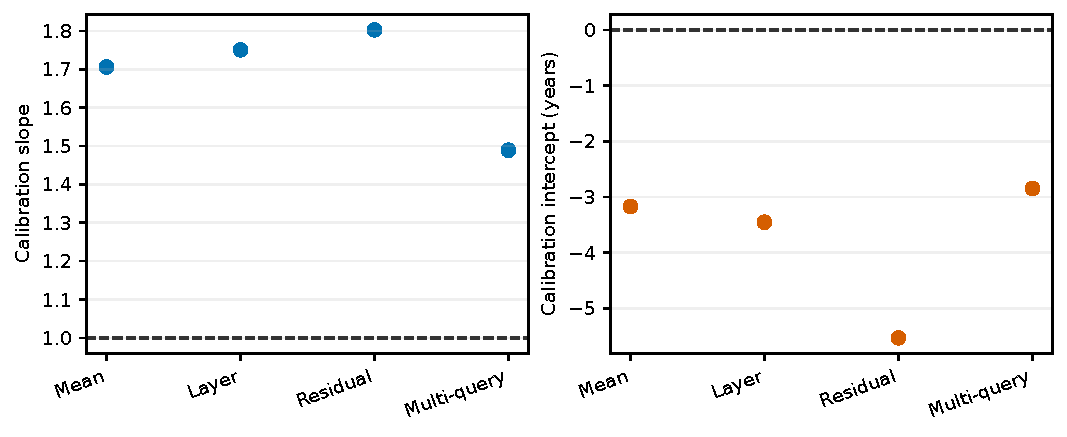
\includegraphics[width=0.80\linewidth]{generated/calibration_summary.pdf}
  \caption{Mean MIPDB calibration slopes and intercepts across seeds. Dashed
  lines mark one and zero, respectively. Calibration regresses observed age on
  predicted age; no external recalibration was applied.}
  \label{fig:calibration}
\end{figure}

\begin{figure}[!htbp]
  \centering
  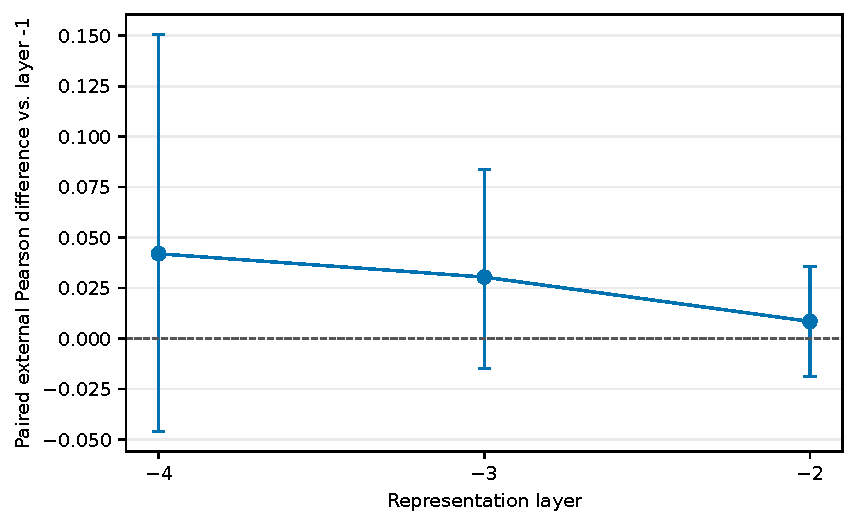
\includegraphics[width=0.80\linewidth]{../results/extensions/layerwise_probe_20260910/assets/layerwise_depth.pdf}
  \caption{Exploratory layer-wise differences from the final layer, with joint
  seed-and-participant intervals. All intervals include zero.}
  \label{fig:layerwise-depth}
\end{figure}

\begin{figure}[!htbp]
  \centering
  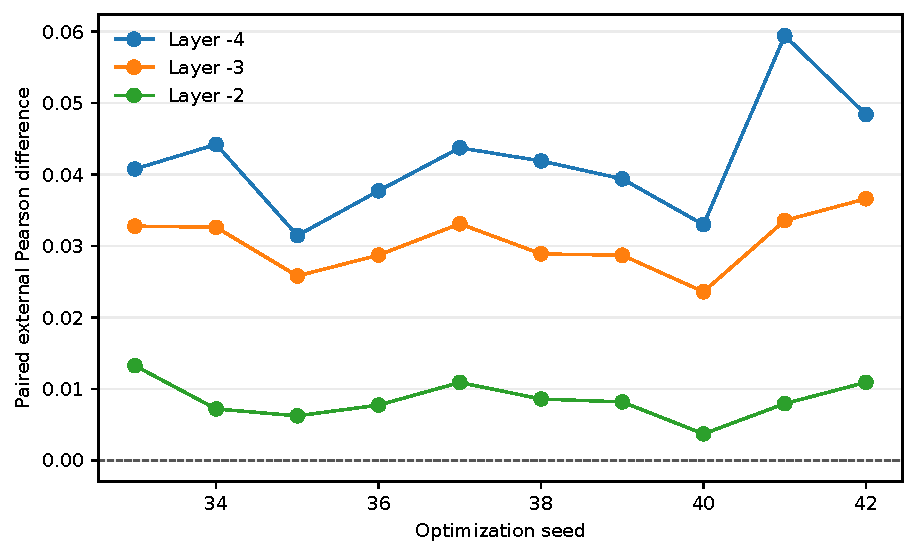
\includegraphics[width=0.80\linewidth]{../results/extensions/layerwise_probe_20260910/assets/layerwise_seed_deltas.pdf}
  \caption{Paired layer-wise Pearson differences across seeds on the same
  MIPDB participants.}
  \label{fig:layerwise-seed-deltas}
\end{figure}

\clearpage
\section{Training-Size Analysis}
\label{sec:capacity}

This exploratory analysis used three heads, three nested HBN training subsets,
and ten seeds, for 90 runs. Each selected checkpoint was evaluated on the same
75 MIPDB participants. The resulting 6,750 predictions are repeated evaluations
of those participants, not independent observations.

\subsection{Absolute performance and paired differences}
Table~\ref{tab:capacity-absolute} reports absolute correlations and parameter
counts. Table~\ref{tab:capacity-cells} gives candidate differences from the
size-matched baseline. The richer heads improved on all ten seeds in each cell.
Both 200-subject intervals and the MLP's 400-subject interval excluded zero;
the other intervals included zero.

\begin{table}[!htbp]
  \centering
  \small
  \caption{MIPDB correlations by HBN training size. SD is computed across ten
  seeds. The MLP has four hidden units.}
  \label{tab:capacity-absolute}
  \begin{tabular}{llrrr}
\toprule
Train $n$ & Head & Params & Mean Pearson & Seed SD \\
\midrule
200 & Mean-linear baseline & 513 & 0.527 & 0.011 \\
200 & Rich statistics & 2561 & 0.604 & 0.009 \\
200 & MLP (4 units) & 2569 & 0.582 & 0.025 \\
400 & Mean-linear baseline & 513 & 0.655 & 0.008 \\
400 & Rich statistics & 2561 & 0.711 & 0.008 \\
400 & MLP (4 units) & 2569 & 0.704 & 0.014 \\
800 & Mean-linear baseline & 513 & 0.645 & 0.008 \\
800 & Rich statistics & 2561 & 0.676 & 0.007 \\
800 & MLP (4 units) & 2569 & 0.662 & 0.012 \\
\bottomrule
\end{tabular}

\end{table}

\begin{table}[!htbp]
  \centering
  \small
  \caption{Paired candidate differences at each training size. W/T/L counts
  positive, zero, and negative seed differences. Intervals resample seeds and
  participants; p-values are exploratory.}
  \label{tab:capacity-cells}
  \begin{tabular}{rlrrrrr}
\toprule
Train $n$ & Head & Params & Mean $\Delta$ & 95\% CI & Holm $p$ & W/T/L \\
\midrule
200 & Rich statistics & 2561 & 0.078 & [0.019, 0.138] & 0.006 & 10/0/0 \\
400 & Rich statistics & 2561 & 0.056 & [-0.017, 0.139] & 0.006 & 10/0/0 \\
800 & Rich statistics & 2561 & 0.031 & [-0.048, 0.120] & 0.006 & 10/0/0 \\
200 & MLP (4 units) & 2569 & 0.056 & [0.019, 0.097] & 0.006 & 10/0/0 \\
400 & MLP (4 units) & 2569 & 0.049 & [0.006, 0.096] & 0.006 & 10/0/0 \\
800 & MLP (4 units) & 2569 & 0.017 & [-0.040, 0.076] & 0.006 & 10/0/0 \\
\bottomrule
\end{tabular}

\end{table}

\subsection{Changes in the candidate advantage}
Table~\ref{tab:capacity-contrasts} compares paired advantages between training
sizes. For example, 800 minus 200 subtracts the candidate's advantage at 200
subjects from its advantage at 800. All observed changes were negative. The
one-sided sign-flip tests retained the prespecified positive-change alternative,
which explains their large p-values; they are not tests for any change in
either direction. Only the MLP's 800-minus-400 bootstrap interval excluded zero.
The endpoint intervals included zero for both heads.

\begin{table}[!htbp]
  \centering
  \small
  \caption{Exploratory changes in the paired Pearson advantage. A negative
  value means a smaller candidate advantage at the larger training size.
  Holm p-values test the positive direction; SD describes seed differences.}
  \label{tab:capacity-contrasts}
  \begin{tabular}{llrrrr}
\toprule
Head & Contrast & Change in $\Delta$ & 95\% CI & Holm $p$ & SD \\
\midrule
Rich statistics & 800 minus 200 & -0.046 & [-0.112, 0.023] & 1.000 & 0.010 \\
Rich statistics & 400 minus 200 & -0.022 & [-0.069, 0.031] & 1.000 & 0.008 \\
Rich statistics & 800 minus 400 & -0.024 & [-0.065, 0.016] & 1.000 & 0.005 \\
MLP (4 units) & 800 minus 200 & -0.039 & [-0.090, 0.012] & 1.000 & 0.018 \\
MLP (4 units) & 400 minus 200 & -0.007 & [-0.044, 0.029] & 1.000 & 0.014 \\
MLP (4 units) & 800 minus 400 & -0.032 & [-0.061, -0.004] & 1.000 & 0.008 \\
\bottomrule
\end{tabular}

\end{table}

Table~\ref{tab:capacity-transfer} shows HBN validation and MIPDB correlations for
the selected candidate checkpoints. External scores did not select checkpoints.
Figure~\ref{fig:capacity-absolute} shows absolute performance, and
Figure~\ref{fig:capacity-seed-deltas} shows individual seed differences.
The joint intervals are shown once in Figure~\ref{fig:capacity-main}.

\begin{table}[!htbp]
  \centering
  \small
  \caption{HBN validation and MIPDB correlations for selected candidate heads,
  averaged over seeds.}
  \label{tab:capacity-transfer}
  \begin{tabular}{llrr}
\toprule
Train $n$ & Head & HBN validation $r$ & MIPDB $r$ \\
\midrule
200 & Rich statistics & 0.645 & 0.604 \\
400 & Rich statistics & 0.711 & 0.711 \\
800 & Rich statistics & 0.736 & 0.676 \\
200 & MLP (4 units) & 0.648 & 0.582 \\
400 & MLP (4 units) & 0.741 & 0.704 \\
800 & MLP (4 units) & 0.742 & 0.662 \\
\bottomrule
\end{tabular}

\end{table}

\begin{figure}[!htbp]
  \centering
  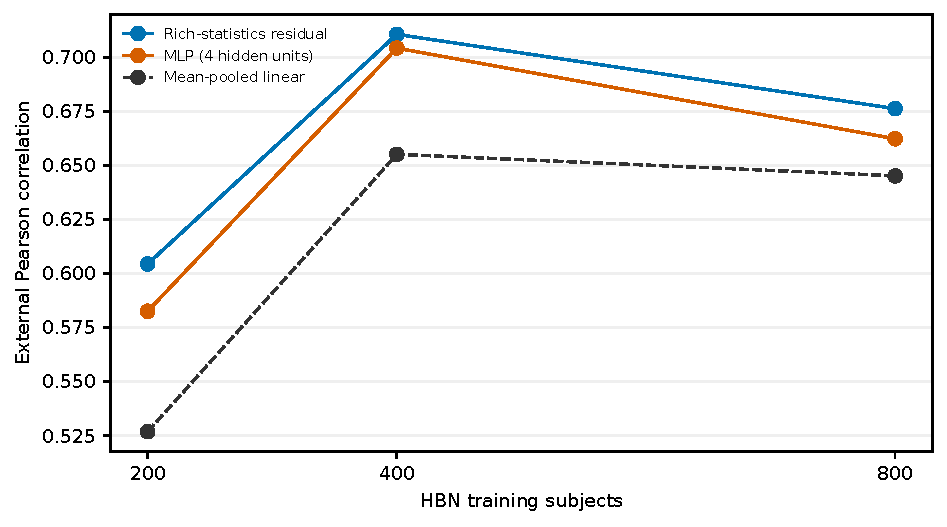
\includegraphics[width=0.80\linewidth]{presentation/capacity_data_regime_absolute.pdf}
  \caption{Absolute MIPDB correlations for each training size and head.}
  \label{fig:capacity-absolute}
\end{figure}

\begin{figure}[!htbp]
  \centering
  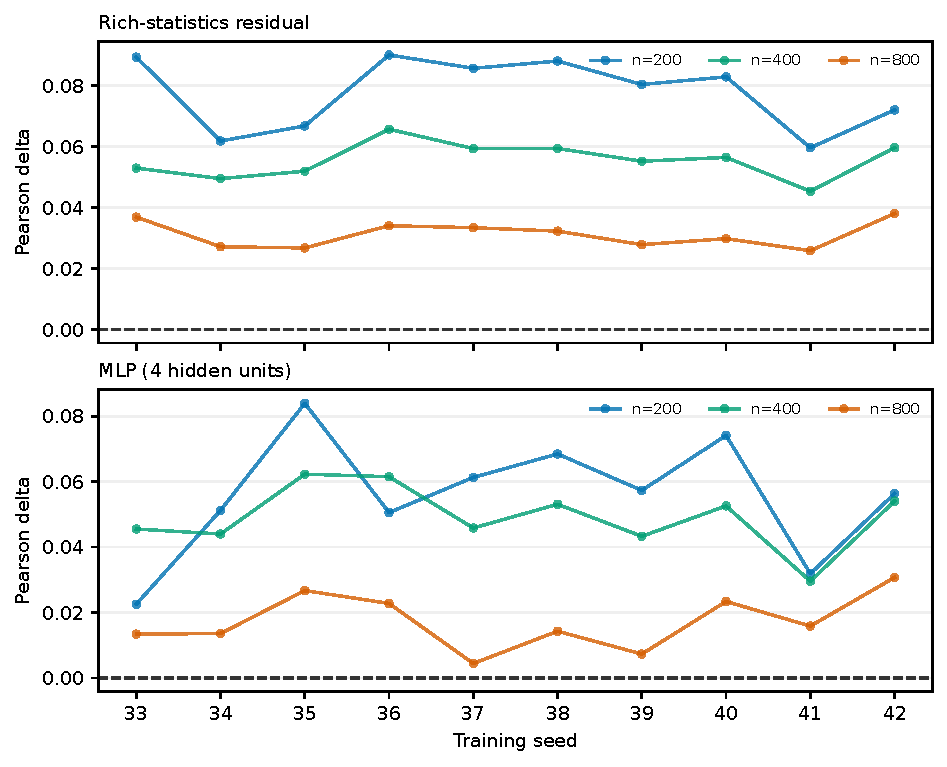
\includegraphics[width=0.80\linewidth]{presentation/capacity_data_regime_seed_deltas.pdf}
  \caption{Paired Pearson differences for the rich-statistics and four-unit
  MLP heads across seeds and HBN training sizes.}
  \label{fig:capacity-seed-deltas}
\end{figure}

